\documentclass[12pt, oneside]{article}

\usepackage[letterpaper, scale=0.8, centering]{geometry}
\usepackage{fancyhdr}
\setlength{\parindent}{0em}
\setlength{\parskip}{1em}

\pagestyle{fancy}
\fancyhf{}
\renewcommand{\headrulewidth}{0pt}
\rfoot{{\footnotesize Copyright Mia Minnes, 2025, Version \today~(\thepage)}}

\usepackage{titlesec}

\author{CSE105W25}

\newcommand{\instructions}{{\bf For all HW assignments:} Weekly homework 
may be done individually or in groups of up to 3 students. 
You may switch HW partners for different HW assignments. 
Please ensure your name(s) and PID(s) are clearly visible on the first page of your homework submission 
and then upload the PDF to Gradescope. If working in a group, submit only one submission per group: 
one partner uploads the submission through their Gradescope account and then adds the other group member(s) 
to the Gradescope submission by selecting their name(s) in the ``Add Group Members" dialog box. 
You will need to re-add your group member(s) every time you resubmit a new version of your assignment.
 Each homework question will be graded either for correctness (including clear and precise explanations and 
 justifications of all answers) or fair effort completeness. 
 On the ``graded for correctness"
 questions, you may only collaborate with CSE 105 students in your group; if your
 group has questions about a problem, you may ask in drop-in help hours or post a private
post (visible only to the Instructors) on Piazza. On the "graded for completeness" questions, you 
may collaborate with all other CSE 105 students this quarter, and you may make public posts about these questions 
on Piazza.

All submitted homework for this class must be typed. 
You can use a word processing editor if you like (Microsoft Word, Open Office, Notepad, Vim, Google Docs, etc.) 
but you might find it useful to take this opportunity to learn LaTeX. 
LaTeX is a markup language used widely in computer science and mathematics. 
The homework assignments are typed using LaTeX and you can use the source files 
as templates for typesetting your solutions.
To generate state diagrams of machines, you can (1) use the LaTex tikzpicture
environment (see templates in the class notes), or (2) use the software tools Flap.js or
JFLAP described in the class syllabus (and include a screenshot in your PDF), or (3) you can carefully
and clearly hand-draw
the diagram and take a picture and include it in your PDF.
We recommend that you
submit early drafts to Gradescope so that in case of any technical difficulties, at least some of your
work is present. You may update your submission as many times as you'd like up to the deadline.


{\bf Integrity reminders}
\begin{itemize}
\item Problems should be solved together, not divided up between the partners. The homework is
designed to give you practice with the main concepts and techniques of the course, 
while getting to know and learn from your classmates.
\item On the "graded for correctness"
questions, you may only collaborate with CSE 105 students in your group.
You may ask questions about the homework in office hours (of the instructor, TAs, and/or tutors) and 
on Piazza (as private notes viewable only to the Instructors).  
You \emph{cannot} use any online resources about the course content other than the class material 
from this quarter -- this is primarily to ensure that we all use consistent notation and
definitions (aligned with the textbook) and also to protect the learning experience you will have when
the `aha' moments of solving the problem authentically happen.
\item Do not share written solutions or partial solutions for homework with 
other students in the class who are not in your group. Doing so would dilute their learning 
experience and detract from their success in the class.
\end{itemize}

}

\newcommand{\gradeCorrect}{({\it Graded for correctness}) }
\newcommand{\gradeCorrectFirst}{\gradeCorrect\footnote{This means your solution 
will be evaluated not only on the correctness of your answers, but on your ability
to present your ideas clearly and logically. You should explain how you 
arrived at your conclusions, using
mathematically sound reasoning. Whether you use formal proof techniques or 
write a more informal argument
for why something is true, your answers should always be well-supported. 
Your goal should be to convince the
reader that your results and methods are sound.} }
\newcommand{\gradeComplete}{({\it Graded for completeness}) }
\newcommand{\gradeCompleteFirst}{\gradeComplete\footnote{This means you will 
get full credit so long as your submission demonstrates honest effort to 
answer the question. You will not be penalized for incorrect answers. 
To demonstrate your honest effort in answering the question, we 
expect you to include your attempt to answer *each* part of the question. 
If you get stuck with your attempt, you can still demonstrate 
your effort by explaining where you got stuck and what 
you did to try to get unstuck.} }

\usepackage{tikz}
\usetikzlibrary{automata,positioning,arrows}

\input{../../resources/discrete-math-packages}

\newcommand{\SUBSTRING}{\textsc{Substring}}
\newcommand{\REP}{\textsc{Rep}}
\newcommand{\blank}{\scalebox{1.5}{\textvisiblespace}}


\title{HW1CSE105W25: Homework assignment 1}
\date{Due: January 16th at 5pm, via Gradescope}


\begin{document}
\maketitle
\thispagestyle{fancy}

{\bf In this assignment,}

You will practice reading and
applying the definitions of alphabets, strings, languages, Kleene star, and regular expressions.
You will use regular expressions and relate them to languages and finite automata.
You will use precise notation to formally define the state diagram of finite automata,
and you will use clear English to describe computations of finite automata informally.


{\bf Resources}: To review the topics 
for this assignment, see the class material from Weeks 0 and 1.
We will post frequently asked questions and our answers to them in a 
pinned Piazza post.

{\bf Reading and extra practice problems}: Sipser Section 0, 1.3, 1.1.
Chapter 1 exercises 1.1, 1.2, 1.3, 1.18, 1.23.

\instructions

You will submit this assignment via Gradescope
(\href{https://www.gradescope.com}{https://www.gradescope.com}) 
in the assignment called ``hw1CSE105W25''.

{\bf Assigned questions}

(To be updated soon)
\end{document}

\begin{enumerate}[wide, labelwidth=!, labelindent=0pt]
%%%%%%%%%%% PROBLEM 1 %%%%%%%%%%%
\item\textbf{Finding examples and edge cases} (12 points):

With $\Sigma= \{0,1,2,3,4,5,6,7,8,9\}$
and $\Gamma = \{0,1,2, 3, 4, 5,6, 7, 8, 9, A, B, C, D, E, F\}$

    \begin{enumerate}
    \item\gradeCompleteFirst  Give an example of a string over $\Sigma$ that is meaningful to you in some way
    and whose length is between $5$ and $20$, and explain 
    why this string is meaningful to you.

    \item\gradeComplete Calculate the number of distinct strings of length 3 over $\Sigma$ and then 
     explain your calculation.

    \item\gradeComplete With the ordering $0 < 1 < 2 < 3 < 4< 5< 6< 7 < 8 < 9< A < B < C < D< E< F$, 
    list the first 50 strings over $\Gamma$ in string order. Explain how you constructed this list.
    {\it Note: you can write a program
    to generate this list if you'd like, and you may use any external tools to help you write this program.
    If you do use a program to generate the list, include it (and documentation for how it works) as part of your
    submission.}

    \item\gradeCorrectFirst Give an example of a finite set that is a language over $\Sigma$ and over $\Gamma$, 
    or explain why there is no such set. A complete and correct answer will use clear and precise notation 
    (consistent with the textbook and class notes) and will include a description of why the given example 
    is a language over $\Sigma$ and over $\Gamma$ and is finite, or an explanation why there is no such example.
    
    \item\gradeCorrect Give an example of an infinite set that is a language over $\Sigma$  and not over $\Gamma$, 
    or explain why there is no such set. A complete and correct answer will use clear and precise notation
    (consistent with the textbook and class notes) and will include a description of why the given example 
    is a language over $\Sigma$ and not over $\Gamma$ and is infinite, or an explanation why there is no such example.

    \end{enumerate}

%%%%%%%%%%% PROBLEM 2 %%%%%%%%%%%
\item\textbf{Regular expressions} (10 points):

    \begin{enumerate}
    \item\gradeComplete  Give three regular expressions that all describe the set of all strings over $\{a,b\}$ that have 
    odd length. Ungraded bonus challenge: Make the expressions as different as possible!

    \item\gradeComplete  A friend tells you that each regular expression that has a Kleene star ($~^*$) describes an
    infinite language. Are they right? Either help them justify their claim or give a counterexample to disprove it
    and explain your counterexample.

    \end{enumerate}

%%%%%%%%%%% PROBLEM 3 %%%%%%%%%%%
\item\textbf{Functions over languages} (15 points):

For each language $L$ over the alphabet $\Sigma_1 = \{0,1\}$, we have the 
associated sets of strings
\[
    SUBSTRING(L) = \{ w \in \Sigma_1^* ~|~ \text{there exist } x,y \in \Sigma_1^* \text{ such that } xwy \in L\}
\]
and 
\[
    EXTEND(L) = \{ w \in \Sigma_1^* ~|~ w = uv \text{ for some strings } u \in L \text{ and } v \in \Sigma_1^* \}
\]
    \begin{enumerate}
    \item\gradeComplete Specify an example language $A$ over $\Sigma_1$ such that 
    $SUBSTRING(A) = EXTEND(A)$, 
    or explain why there is no such example. 
    A complete solution will include either (1) a precise and
    clear description of your example language $A$ 
    and a precise and clear description of
    the result of computing $SUBSTRING(A)$, $EXTEND(A)$ (using the given definitions)
    to justify this description and to justify the set equality,
    or (2) a sufficiently general and correct argument
    why there is no such example, referring back to the relevant definitions.

    \item\gradeCorrect Specify an example language $B$ over $\Sigma_1$ such that 
    $$SUBSTRING(B) = \{\varepsilon\}$$ and $$EXTEND(B) = \Sigma_1^*$$
    or explain why there is no such example. 
    A complete solution will include either (1) a precise and
    clear description of your example language $B$ 
    and a precise and clear description of
    the result of computing $SUBSTRING(B)$, $EXTEND(B)$ (using the given definitions)
    to justify this description and to justify the set equality with 
    $\{\varepsilon\}$ and $\Sigma_1^*$ (respectively), or (2) a sufficiently general and correct argument
    why there is no such example, referring back to the relevant definitions.

    \item\gradeCorrect Specify an example {\bf infinite} language $C$ over $\Sigma_1$ such that 
    $$SUBSTRING(C) \neq \Sigma_1^*$$ and $$EXTEND(C) \neq \Sigma_1^*$$, or 
    explain why there is no such example.
    A complete solution will include either (1) a precise and
    clear description of your example language $C$ 
    and a precise and clear description of
    the result of computing $SUBSTRING(B)$, $EXTEND(B)$ (using the given definitions)
    to justify this description and to justify the set nonequality claims, 
    or (2) a sufficiently general and correct argument
    why there is no such example, referring back to the relevant definitions.
    \end{enumerate}


%%%%%%%%%%% PROBLEM 4 %%%%%%%%%%%
\item\textbf{Finite automata} (13 points):

Consider the finite automaton $(Q, \Sigma, \delta, q_0, F)$ whose state diagram is depicted below
\begin{center}
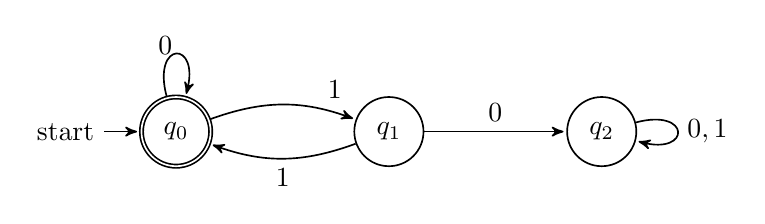
\begin{tikzpicture}[->,>=stealth',shorten >=1pt, auto, node distance=2cm, semithick]
\tikzstyle{every state}=[text=black, fill=none]

\node[initial,state, accepting] (q0)          {$q_0$};
\node[state]         (q1) [right of=q0, xshift=20pt] {$q_1$};
\node[state]         (q2) [right of=q1, xshift=20pt] {$q_2$};

\path (q0) edge  [loop above, near start] node {$0$} (q0)
        edge [bend left=20, near end] node {$1$} (q1)
    (q1) edge [bend left=0] node {$0$} (q2)
        edge [bend left=20] node {$1$} (q0)
    (q2) edge [loop right] node {$0,1$} (q2)
;
\end{tikzpicture}
\end{center}
where $Q = \{q_0, q_1, q_2\}$, $\Sigma = \{0,1\}$, and $F = \{q_0\}$, and $\delta: Q \times \Sigma \to Q$
is specified by the look-up table
\begin{center}
\begin{tabular}{c|cc}
        & $0$ & $1$ \\
    \hline
  $q_0$ & $q_0$ & $q_1$ \\
  $q_1$ & $q_2$ & $q_0$ \\
  $q_2$ & $q_2$ & $q_2$
\end{tabular}
\end{center}
    \begin{enumerate}
    \item\gradeComplete A friend tries to summarize the transition function with the formula
    \[
        \delta(q_i,x) = \begin{cases}
            q_0 &\text{ when $i=0$ and $x=0$} \\
            q_2 &\text{ when $x < i$}\\
            q_j &\text{ when $j = (i+1) \mod 2$ and $x=1$}
        \end{cases}
    \]
    for $x \in \{0,1\}$ and $i \in \{0,1,2\}$.
    Are they right? Either help them justify their claim or give a counterexample to disprove it and then 
    fix their formula.

    \item\gradeCorrect Give a regular expression $R$ so that $L(R)$ is the language 
    recognized by this finite automaton. Justify your answer by referring to the 
    definition of the semantics of regular expressions and computations of finite automata. 
    Include an explanation for why each string in $L(R)$ is accepted by the finite automaton {\it and}
    for why each string not in $L(R)$ is rejected by the finite automaton.

    \item\gradeCorrect Keeping the same set of states $Q = \{q_0, q_1, q_2\}$, alphabet $\Sigma = \{0,1\}$, 
    same start state $q_0$, and same transition 
    function $\delta$, choose a new set of accepting states $F_{new}$ so that the new 
    finite automaton that results accepts at least one string that the original one rejected {\bf and} rejects
    at least one string that the original one accepted, or explain why there is no such choice of $F_{new}$.
    A complete solution will include either (1) a precise and
    clear description of your choice of $F_{new}$
    and a precise and clear the two example strings using relevant definitions 
    to justify them, or (2) a sufficiently general and correct argument
    why there is no such example, referring back to the relevant definitions.

    \end{enumerate}
    
    \end{enumerate}
\end{document}